\documentclass[12pt,a4paper]{article}

% =========================================================================
% FORMATAÇÃO ABNT (NBR 14724 / NBR 6024 / NBR 6027)
% =========================================================================

% --- Margens ABNT (3 cm superior e esquerda; 2 cm inferior e direita) ---
\usepackage[
  a4paper,
  left=3cm,
  top=3cm,
  right=2cm,
  bottom=2cm,
  headheight=15pt,
  headsep=1cm
]{geometry}

% --- Idioma, codificação e tipografia (Times New Roman - ABNT NBR 14724) ---
\usepackage[T1]{fontenc}
\usepackage[utf8]{inputenc}
\usepackage[brazil]{babel}
\usepackage{amsmath}
\usepackage{newtxtext,newtxmath}
\usepackage{microtype}
\usepackage[htt]{hyphenat} % permite quebra de linha em identificadores \texttt

% --- Espaçamento e parágrafo ABNT ---
\usepackage{setspace}
\onehalfspacing                    % 1,5 entre linhas para o texto
\usepackage{indentfirst}           % recuo no primeiro parágrafo
\setlength{\parindent}{1.25cm}     % recuo padrão ABNT
\setlength{\parskip}{0pt}
\setlength{\emergencystretch}{2em} % evita linhas muito longas (overfull hbox)

% --- Tabelas e alinhamentos ---
\usepackage{array}
\usepackage{tabularx}
\usepackage{booktabs}
\usepackage{etoolbox}

% --- Figuras, quadros e imagens ---
\usepackage{graphicx}
\graphicspath{{../assets/}{assets/}}
\usepackage{float}

% --- Cabeçalhos e paginação ABNT (NBR 14724 item 5.3) ---
% Numeração arábica visível no canto superior direito (2 cm do topo, 2 cm da borda direita).
% Páginas pré-textuais contadas sem numeração aparente.
\usepackage{fancyhdr}
\pagestyle{empty}
\fancyhf{}
\fancyhead[R]{\small\thepage}
\renewcommand{\headrulewidth}{0pt}

% --- Formatação do Sumário (NBR 6027) ---
\usepackage{tocloft}
\renewcommand{\cftsecleader}{\cftdotfill{\cftdotsep}}
\renewcommand{\cftsecfont}{\bfseries}
\renewcommand{\cftsecpagefont}{\bfseries}
\setlength{\cftbeforesecskip}{0.4em}

% --- Formatação dos títulos de seções (NBR 6024) ---
\usepackage{titlesec}
% 1 SEÇÃO PRIMÁRIA (caixa alta, negrito)
\titleformat{\section}
  {\normalfont\normalsize\bfseries\MakeUppercase}{\thesection}{1em}{}
% 1.1 Seção secundária (negrito)
\titleformat{\subsection}
  {\normalfont\normalsize\bfseries}{\thesubsection}{1em}{}
% 1.1.1 Seção terciária (negrito)
\titleformat{\subsubsection}
  {\normalfont\normalsize\bfseries}{\thesubsubsection}{1em}{}
% 1.1.1.1 Seção quaternária (itálico)
\titleformat{\paragraph}
  {\normalfont\normalsize\itshape}{\theparagraph}{1em}{}

\titlespacing*{\section}{0pt}{2ex plus 0.5ex minus 0.2ex}{1.5ex plus 0.5ex minus 0.2ex}
\titlespacing*{\subsection}{0pt}{1.8ex plus 0.5ex minus 0.2ex}{1.2ex plus 0.5ex minus 0.2ex}
\titlespacing*{\subsubsection}{0pt}{1.5ex plus 0.5ex minus 0.2ex}{1.0ex plus 0.5ex minus 0.2ex}

% --- Legendas e fontes (NBR 14724 / IBGE) ---
\usepackage{caption}
\captionsetup{
  font=small,
  labelfont=bf,
  justification=centering,
  singlelinecheck=false,
  skip=6pt
}
\captionsetup[figure]{name=Figura, labelsep=endash}
\captionsetup[table]{name=Quadro, labelsep=endash}

% "Fonte:" abaixo de figuras e quadros
\newcommand{\fonte}[1]{%
  \par\vspace{2pt}%
  {\footnotesize\raggedright\textbf{Fonte:} #1\par}%
}

% Espaçamento simples dentro de figuras e quadros (exigência ABNT)
\AtBeginEnvironment{figure}{\singlespace}
\AtBeginEnvironment{table}{\singlespace}

% --- Códigos-fonte (PlantUML) ---
\usepackage{xcolor}
\usepackage{listings}
% pdfLaTeX: converte UTF-8 -> latin1 nos listings (garante acentuação correta)
\ifdefined\pdftexversion
  \usepackage{listingsutf8}
\fi
\definecolor{codgray}{gray}{0.45}
\lstset{
  basicstyle=\ttfamily\footnotesize,
  breaklines=true,
  columns=fullflexible,
  keepspaces=true,
  showstringspaces=false,
  frame=single,
  framexleftmargin=4pt,
  tabsize=2,
  numbers=left,
  numberstyle=\tiny\color{codgray},
  numbersep=8pt,
  xleftmargin=20pt,
  captionpos=b
}
% pdfLaTeX precisa decodificar UTF-8 explicitamente nos listings
\ifdefined\pdftexversion
  \lstset{inputencoding=utf8/latin1, extendedchars=true}
\fi

% --- Listas compactas ---
\providecommand{\tightlist}{%
  \setlength{\itemsep}{0pt}\setlength{\parskip}{0pt}}

% --- Links e marcadores ---
\usepackage[hidelinks]{hyperref}
\usepackage{bookmark}
\IfFileExists{xurl.sty}{\usepackage{xurl}}{}
\urlstyle{same}

\begin{document}

% =========================================================================
% ELEMENTOS PRÉ-TEXTUAIS (NBR 14724)
% =========================================================================

% --- CAPA ---
\begin{titlepage}
  \thispagestyle{empty}
  \begin{center}
    \textbf{\large UNIVERSIDADE FEDERAL DE GOIÁS}\\[0.2cm]
    \textbf{\large INSTITUTO DE INFORMÁTICA}\\[0.2cm]
    \textbf{\large BACHARELADO EM ENGENHARIA DE SOFTWARE}\\[0.2cm]
    \textbf{\large DISCIPLINA: MODELAGEM DE SOFTWARE}

    \vspace{3.2cm}
    {\large
    Carlos Eduardo Freire da Silva\\
    Gabriel Henrique Lourenço Dias\\
    Kayque Vicente Silva\\
    Luiz Pedro Pereira Mendes Saraiva\\
    Yury Nogueira de Oliveira Silva\par}

    \vspace{3.5cm}
    \textbf{\Large SISTEMA DE AGENDAMENTO DE CONSULTAS MÉDICAS}\\[0.4cm]
    \textbf{\large Modelagem de Software --- APS 1}\par

    \vfill
    \textbf{GOIÂNIA}\\[0.2cm]
    \textbf{2026}
  \end{center}
\end{titlepage}

% --- FOLHA DE ROSTO ---
\thispagestyle{empty}
\begin{center}
  {\large
  Carlos Eduardo Freire da Silva\\
  Gabriel Henrique Lourenço Dias\\
  Kayque Vicente Silva\\
  Luiz Pedro Pereira Mendes Saraiva\\
  Yury Nogueira de Oliveira Silva\par}

  \vspace{4.0cm}
  \textbf{\Large SISTEMA DE AGENDAMENTO DE CONSULTAS MÉDICAS}\\[0.4cm]
  \textbf{\large Modelagem de Software --- APS 1}\par
\end{center}

\vspace{2.5cm}
\begin{flushright}
  \begin{minipage}{0.52\textwidth}
    \begin{singlespace}
      {\small Trabalho acadêmico apresentado à disciplina de Modelagem
      de Software do curso de Bacharelado em Engenharia de Software da
      Universidade Federal de Goiás (UFG), como requisito parcial de
      avaliação referente à Atividade Prática Supervisionada (APS
      1).\\[0.4cm]
      \textbf{Professor Orientador:} Prof. Me. Diogo Oliveira Santos}
    \end{singlespace}
  \end{minipage}
\end{flushright}

\vfill
\begin{center}
  \textbf{GOIÂNIA}\\[0.2cm]
  \textbf{2026}
\end{center}
\newpage

% --- SUMÁRIO (NBR 6027) ---
\thispagestyle{empty}
\renewcommand{\contentsname}{SUMÁRIO}
\pdfbookmark[0]{\contentsname}{toc}
\tableofcontents
\newpage

% =========================================================================
% ELEMENTOS TEXTUAIS (início da numeração de página visível - NBR 14724)
% =========================================================================

\pagestyle{fancy}
\thispagestyle{fancy}

\section{Descrição da Aplicação}\label{sec:descricao}

\subsection{Contexto e Objetivos}\label{sec:contexto}

Este trabalho apresenta a modelagem de um sistema web para utilização
em clínicas e consultórios, que permite que os usuários realizem
agendamentos de consultas e, para a clínica, o gerenciamento da agenda
de atendimento de diversos médicos e suas especialidades.

Temos como objetivo principal dar autonomia ao usuário para que ele
consiga, a qualquer momento, realizar um agendamento na clínica
desejada, selecionando a especialidade e o médico e definindo o horário,
sem precisar fazer ligações ou enviar mensagens, agilizando assim o
processo de agendamento, remarcação e cancelamento de consultas. Além
disso, a equipe da clínica passa a ter um melhor gerenciamento da agenda
de seus médicos especialistas, ganhando agilidade no processo e
permitindo que os próprios médicos cadastrem seus horários, enquanto o
administrador tem uma visão geral do funcionamento da clínica.

\subsection{Problema de Negócio e Solução Proposta}\label{sec:problema}

Processos manuais em clínicas costumam gerar sobrecarga na recepção,
marcações duplas no mesmo horário e alto índice de faltas pela falta de
lembretes práticos. Além disso, controles em planilhas ou papel
dificultam o remanejamento rápido de horários cancelados e não oferecem
histórico confiável para auditoria.

O sistema resolve esses problemas ao centralizar as agendas em uma base
única, aplicando validação em tempo real e bloqueio de horários para
impedir conflitos entre pacientes que desejam um mesmo horário. Para
reduzir as faltas, a aplicação envia confirmações e lembretes
simultaneamente por e-mail e WhatsApp, os dois canais mais usados no dia
a dia. Além disso, todas as ações críticas (agendamentos, confirmações,
cancelamentos e remarcações com motivo obrigatório e alterações de
grade) geram registros de auditoria com autor, data/hora, IP e
navegador, apoiando a rastreabilidade e a conformidade com a LGPD. Ao
armazenar o motivo de cada cancelamento ou remarcação, cria-se um histórico
que ajuda a clínica a entender por que os horários são liberados.

\subsection{Atores do Sistema}\label{sec:atores}

O sistema conta com cinco atores bem definidos:

\begin{enumerate}
\tightlist
\item
  \textbf{Paciente:} cadastra-se com CPF, e-mail e telefone celular;
  autentica-se com senha segura; pesquisa médicos por especialidade;
  consulta a grade de horários disponíveis; e gerencia suas consultas
  (agendamento, histórico, remarcação e cancelamento). Recebe
  notificações automáticas por e-mail e WhatsApp, inclusive um lembrete
  24 horas antes da consulta.
\item
  \textbf{Médico:} profissional cadastrado com CRM, UF e especialidades
  ativas. Configura sua disponibilidade semanal (dias de atendimento,
  horário de expediente e duração das consultas); bloqueia horários
  pontuais por conveniência; visualiza sua agenda; confirma as próprias
  consultas; e registra o status do atendimento (iniciando, concluindo
  ou registrando a ausência do paciente). Não agenda, cancela nem
  remarca consultas.
\item
  \textbf{Secretário:} profissional da recepção. Acompanha as agendas de
  todos os médicos, gerencia as consultas pendentes de confirmação (com
  contato proativo com pacientes quando necessário), registra
  confirmações ou recusas e pode agendar, remarcar ou cancelar consultas
  a pedido de pacientes presenciais ou por telefone.
\item
  \textbf{Administrador:} responsável pelos cadastros dentro do sistema.
  Cadastra e mantém médicos e secretários e gerencia o catálogo de
  especialidades (ativar e desativar). Não agenda nem altera consultas.
\item
  \textbf{Sistema de Notificação:} componente secundário que roda em
  segundo plano. Funciona a partir dos eventos gerados pelas operações
  da clínica e envia as mensagens em paralelo por e-mail e WhatsApp, com
  fila de retentativas automáticas caso ocorra instabilidade temporária
  na rede, garantindo que o agendamento nunca trave por falha de envio.
\end{enumerate}

\subsection{Módulos Funcionais e Regras de Negócio}\label{sec:modulos-regras}

O sistema é organizado em seis módulos complementares:

\begin{itemize}
\tightlist
\item
  \textbf{Módulo de Cadastro e Autenticação:} responsável pelo
  gerenciamento e pela autenticação de todos os usuários da clínica e
  pacientes. Exige e-mail único para todos e CPF único para pacientes.
  Médicos são cadastrados pelo par CRM/UF, dados únicos nacionalmente.
  Os perfis de acesso são exclusivos (\texttt{PACIENTE},
  \texttt{MEDICO}, \texttt{SECRETARIO}, \texttt{ADMINISTRADOR}).
  Pacientes se cadastram sozinhos; médicos e secretários são cadastrados
  pelo administrador. As senhas são armazenadas sob hash criptográfico,
  com bloqueio temporário após sucessivas tentativas incorretas.
\item
  \textbf{Módulo de Consulta de Médicos e Especialidades:} o
  administrador gerencia a lista de especialidades (apenas ativas
  aceitam novos agendamentos). Permite a busca pública de especialidades
  e a filtragem de médicos ativos vinculados a cada catálogo.
\item
  \textbf{Módulo de Agenda do Médico:} organiza a grade do profissional
  em intervalos de \textbf{30 minutos por padrão}, configuráveis pelo
  médico em blocos de 30 minutos, sem sobreposição. Cada intervalo
  possui estado bem definido (\texttt{LIVRE}, \texttt{BLOQUEADO} ou
  \texttt{OCUPADO}). Os horários ficam disponíveis para reserva dentro
  do expediente do médico, respeitando uma antecedência mínima
  configurável e um limite máximo de até 90 dias no futuro. Permite ao
  médico aplicar bloqueios operacionais pontuais.
\item
  \textbf{Módulo de Agendamento:} guia o paciente em quatro passos
  (especialidade, médico, data/horário e confirmação do resumo) e
  centraliza todo o ciclo da reserva. Ao confirmar, o sistema reserva o horário utilizando trava atômica (bloqueio exclusivo no banco de dados) para impedir marcações concorrentes no mesmo slot e grava a consulta como \texttt{AGENDADA}. Abrange também o
  histórico de consultas e as operações de \textbf{cancelamento e
  remarcação} (pelo paciente titular ou pelo secretário): ambas exigem
  antecedência mínima de 2 horas (bloqueando a ação no sistema caso
  falte menos de 2 h) e \textbf{motivo obrigatório}. No cancelamento, o
  slot volta imediatamente a \texttt{LIVRE}. A remarcação mantém o mesmo
  médico, cancelando a consulta antiga, ocupando o novo horário e
  criando uma nova consulta \texttt{AGENDADA} com reversão automática em
  caso de falha.
\item
  \textbf{Módulo de Confirmação (Secretário):} apoia a rotina da
  recepção através de uma visão centralizada das consultas pendentes de
  confirmação. Permite o contato proativo com os pacientes presenciais
  ou telefônicos e o registro de confirmações (transicionando a consulta
  para \texttt{CONFIRMADA}) ou recusas, gravando autor e data da
  confirmação. A confirmação é \textbf{opcional}, permitindo que o
  médico inicie o atendimento mesmo que a consulta permaneça com status
  \texttt{AGENDADA}.
\item
  \textbf{Módulo de Notificação:} funciona em segundo plano, disparando
  avisos assíncronos e em paralelo por e-mail e WhatsApp nos eventos de
  agendamento, confirmação, cancelamento, remarcação e lembrete prévio
  de 24 horas. Cada canal possui registro próprio de entrega com fila de
  até 3 tentativas e backoff. Uma falha de entrega não cancela a consulta
  nem interrompe o fluxo do usuário. Os eventos críticos do sistema são
  registrados em log imutável de auditoria com rastreabilidade de autor,
  data/hora e IP.
\end{itemize}

\subsection{Ciclo de Vida da Consulta}\label{sec:ciclo}

\begin{table}[H]
\centering
\caption{Ciclo de vida da consulta}
\label{qua:ciclo}
{\footnotesize
\begin{tabularx}{\textwidth}{@{}>{\raggedright\arraybackslash}p{2.5cm}>{\raggedright\arraybackslash}p{3.4cm}>{\raggedright\arraybackslash}p{3.2cm}>{\raggedright\arraybackslash}X@{}}
\toprule
De & Evento & Para & Quem pode \\
\midrule
--- & agendar & \texttt{AGENDADA} & Paciente, Secretário \\
\texttt{AGENDADA} & confirmar & \texttt{CONFIRMADA} & Secretário, Médico titular \\
\texttt{AGENDADA}, \texttt{CONFIRMADA} & iniciar & \texttt{EM\_ANDAMENTO} & Médico titular \\
\texttt{AGENDADA}, \texttt{CONFIRMADA} & cancelar ($\geq$ 2 h, com motivo) & \texttt{CANCELADA} & Paciente titular, Secretário \\
\texttt{AGENDADA}, \texttt{CONFIRMADA} & remarcar ($\geq$ 2 h, com motivo) & \texttt{REMARCADA} (e nova \texttt{AGENDADA}) & Paciente titular, Secretário \\
\texttt{AGENDADA}, \texttt{CONFIRMADA} & horário passou sem início & \texttt{NAO\_REALIZADA} & Sistema \\
\texttt{AGENDADA}, \texttt{CONFIRMADA}, \texttt{EM\_ANDAMENTO} & registrar ausência & \texttt{NAO\_REALIZADA} & Médico titular \\
\texttt{EM\_ANDAMENTO} & encerrar & \texttt{REALIZADA} & Médico titular \\
\bottomrule
\end{tabularx}
}
\fonte{Elaborado pelos autores (2026).}
\end{table}

\texttt{CANCELADA}, \texttt{REMARCADA}, \texttt{REALIZADA} e
\texttt{NAO\_REALIZADA} são estados finais de cada consulta.

\newpage
\subsection{Quem Recebe Cada Notificação}\label{sec:notificacoes}

Cada evento gera uma notificação por destinatário e por canal (e-mail e
WhatsApp).

\begin{table}[H]
\centering
\caption{Destinatários das notificações por evento}
\label{qua:notificacoes}
{\footnotesize
\begin{tabularx}{\textwidth}{@{}>{\raggedright\arraybackslash}Xcc@{}}
\toprule
Evento & Paciente & Médico \\
\midrule
Agendamento & sim & não \\
Confirmação & sim & sim \\
Cancelamento & sim & sim \\
Remarcação & sim & sim \\
Lembrete (24 h antes) & sim & não \\
\bottomrule
\end{tabularx}
}
\fonte{Elaborado pelos autores (2026).}
\end{table}

\subsection{Escopo e Premissas}\label{sec:escopo}

\begin{itemize}
\tightlist
\item
  A aplicação é um \textbf{web app responsivo}; não há aplicativo
  nativo.
\item
  Ficam \textbf{fora do escopo}: prontuário eletrônico, prescrições,
  pagamento, convênios, nota fiscal, teleconsulta e várias clínicas
  (multiclínica).
\item
  Há um único contexto de clínica.
\item
  A auditoria cobre eventos de negócio (criar, confirmar, cancelar,
  remarcar, bloquear horário e alterar cadastro), não leituras.
\end{itemize}

\section{Diagramas de Atividades}\label{sec:atividades}

Fizemos um único diagrama de atividades, o \textbf{DA-01}, com o fluxo
principal de agendamento e todos os caminhos alternativos e de erro.
Como ele já cobre o que foi pedido, não criamos diagramas separados para
cancelar, remarcar e confirmar consulta; esses processos estão
explicados nas seções~\ref{sec:modulos-regras} e~\ref{sec:ciclo}.

\subsection{DA-01 --- Agendamento de Consulta}\label{sec:da01}

\textbf{Objetivo:} mostrar o passo a passo do paciente para agendar uma
consulta, do login até receber o comprovante, incluindo o que acontece
quando algo dá errado.

\textbf{Quem participa (raias):} Paciente, Sistema e Sistema de
Notificação.

\textbf{Como funciona:} o paciente faz login (se ainda não estiver
logado), escolhe a especialidade, o médico e um horário livre, confere o
resumo e confirma. O sistema reserva o horário de uma vez só, para dois
pacientes não pegarem a mesma vaga, grava a consulta como
\texttt{AGENDADA}, marca o horário como \texttt{OCUPADO} e registra a
auditoria. Depois disso, o fluxo se divide em duas partes que andam ao
mesmo tempo: o sistema mostra o comprovante ao paciente e o Sistema de
Notificação envia as mensagens. O envio também se divide em dois, e-mail
e WhatsApp, cada um com até 3 tentativas e com seu próprio resultado
(\texttt{ENVIADA} ou \texttt{FALHOU}). No fim tudo se junta, mas o
comprovante não fica esperando o envio.

\begin{figure}[H]
\centering
\caption{DA-01 --- Diagrama de atividades: agendamento de consulta}
\label{fig:da01}
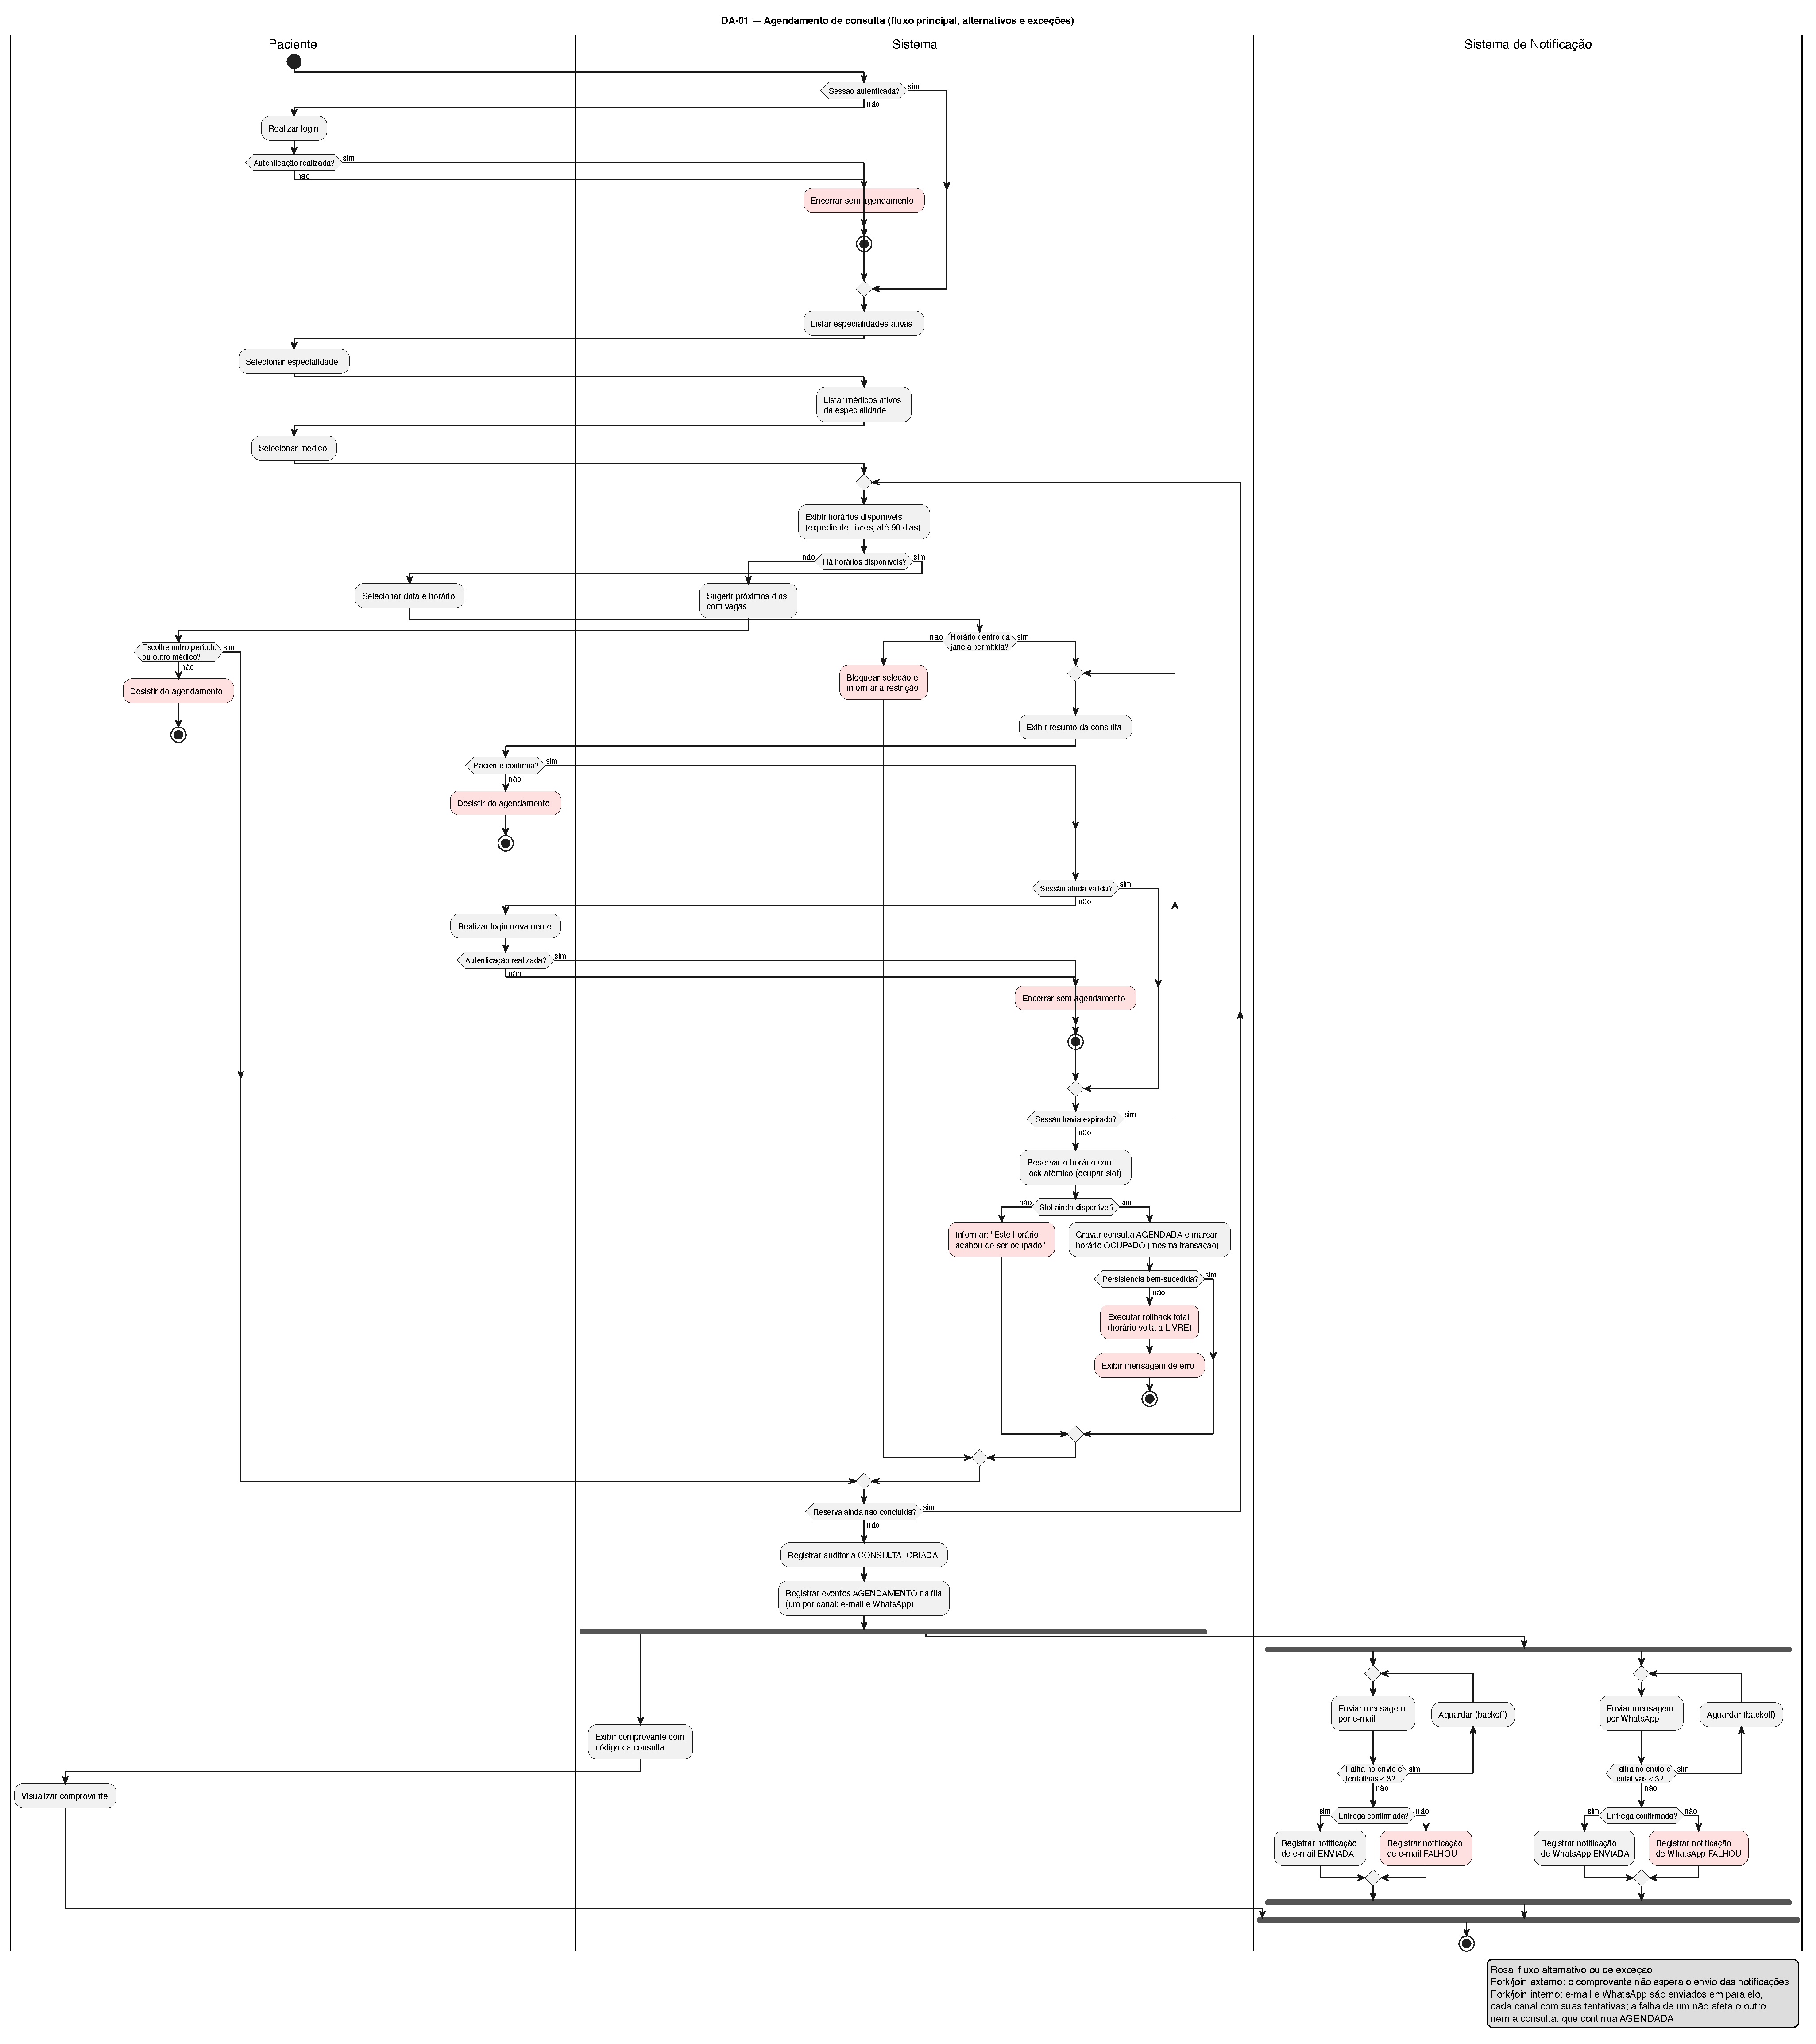
\includegraphics[width=\textwidth,height=0.78\textheight,keepaspectratio]{../assets/DA01_Agendamento.pdf}
\fonte{Elaborado pelos autores (2026).}
\end{figure}

\textbf{Como ler o diagrama:} as raias separam o que cada ator faz. Os
laços (\texttt{repeat}) voltam para a escolha de horário quando não há
vagas, quando o horário está fora da janela ou quando outro paciente
pegou o horário, e voltam para o resumo depois de um novo login. Os
blocos rosa são os caminhos alternativos e de erro. O \emph{fork/join}
mostra o que acontece ao mesmo tempo: o comprovante aparece enquanto as
mensagens são enviadas, e se o envio falhar o agendamento continua
valendo.

\textbf{Onde cada fluxo alternativo (A) e de erro (E) aparece no DA-01:}

\begin{table}[H]
\centering
\caption{Fluxos alternativos e de exceção do DA-01}
\label{qua:fluxos-da01}
{\footnotesize
\begin{tabularx}{\textwidth}{@{}>{\raggedright\arraybackslash}p{4.2cm}>{\raggedright\arraybackslash}X@{}}
\toprule
Fluxo & Onde aparece no diagrama \\
\midrule
Login inicial & No começo, em ``Sessão autenticada?''; se o login falhar, o fluxo termina \\
A1 --- sem horários & ``Há horários disponíveis?'' não $\rightarrow$ o sistema sugere outros dias $\rightarrow$ o paciente escolhe outro período ou médico (volta para a escolha de horário) ou desiste \\
A2 --- horário tomado por outro paciente & ``Slot ainda disponível?'' não $\rightarrow$ aviso ``Este horário acabou de ser ocupado'' $\rightarrow$ volta para a escolha de horário \\
A3 --- falha no envio da mensagem & No Sistema de Notificação: falha no envio $\rightarrow$ até 3 tentativas $\rightarrow$ \texttt{FALHOU}; a consulta continua \texttt{AGENDADA} \\
E1 --- sessão expirou & ``Sessão ainda válida?'' não $\rightarrow$ novo login $\rightarrow$ volta para o resumo da consulta \\
E2 --- falha ao gravar & ``Persistência bem-sucedida?'' não $\rightarrow$ desfaz tudo (o horário volta a \texttt{LIVRE}) $\rightarrow$ mensagem de erro \\
E3 --- horário fora da janela & ``Horário dentro da janela permitida?'' não $\rightarrow$ bloqueia a seleção e explica a restrição \\
Desistências & ``Paciente confirma?'' não, ou ``Escolhe outro período ou outro médico?'' não \\
\bottomrule
\end{tabularx}
}
\fonte{Elaborado pelos autores (2026).}
\end{table}

\section{Diagramas de Sequência}\label{sec:sequencia}

O \textbf{DS-01} cobre o mesmo cenário do DA-01 sob uma perspectiva
diferente: enquanto o diagrama de atividades mapeia \emph{o que}
acontece, o diagrama de sequência revela \emph{como} os participantes se
comunicam para que isso aconteça. Ele ordena cronologicamente as
mensagens trocadas entre o paciente, o sistema, os objetos de negócio
(\texttt{Agenda}, \texttt{Horario}, \texttt{Consulta},
\texttt{Notificacao}) e o Sistema de Notificação, incluindo os retornos
e todos os cenários alternativos e de exceção.

\subsection{DS-01 --- Agendamento de Consulta (Fluxo Completo)}\label{sec:ds01}

\textbf{Objetivo:} documentar, mensagem a mensagem, o que acontece
durante um agendamento. Os pontos centrais são a reserva atômica do
horário --- que previne conflitos de concorrência ---, a criação da
consulta e o rollback em caso de falha, e o envio assíncrono e paralelo
das notificações por e-mail e WhatsApp.

\textbf{Cenário representado:} um paciente autenticado seleciona
especialidade, médico e horário, e conclui o agendamento. O diagrama
trata todas as situações excepcionais relevantes: ausência de horários
disponíveis, seleção de horário fora da janela permitida, sessão
expirada, tentativa de reservar um horário já ocupado por outro
paciente, falha de gravação no banco e falha no envio da notificação.

\begin{figure}[H]
\centering
\caption{DS-01 --- Diagrama de sequência: agendamento de consulta}
\label{fig:ds01}
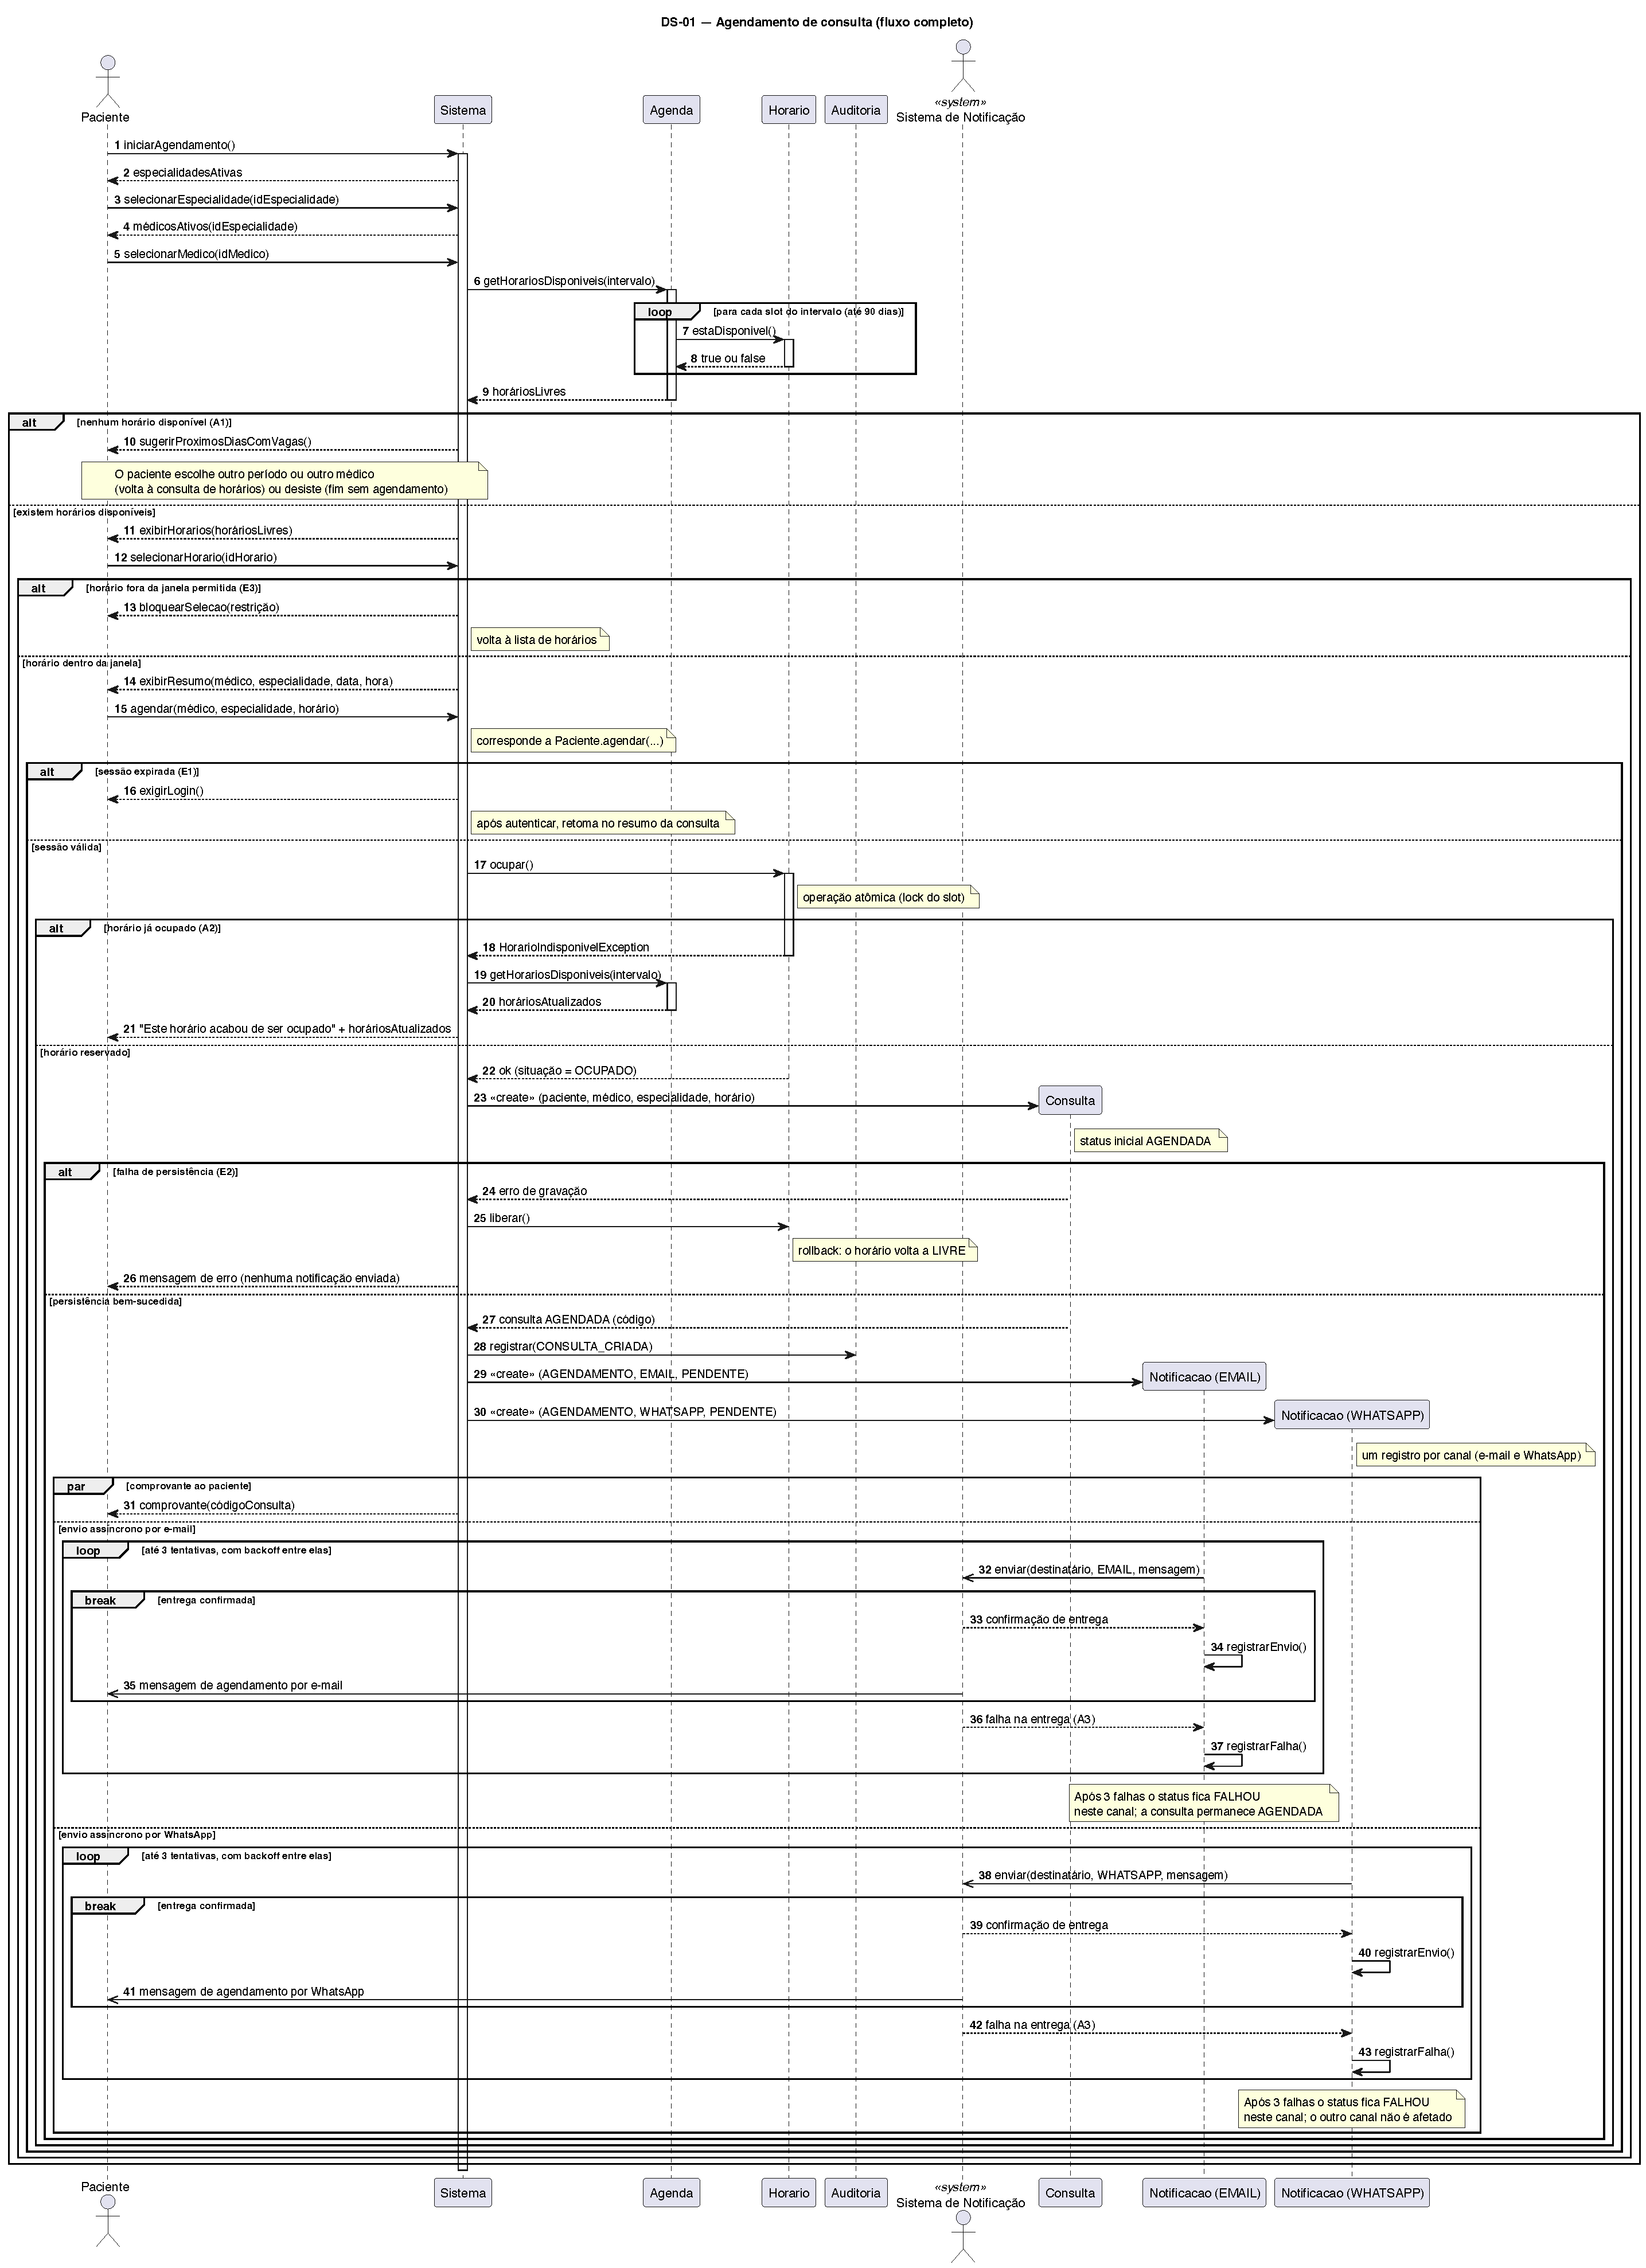
\includegraphics[width=\textwidth,height=0.78\textheight,keepaspectratio]{../assets/DS01_Agendamento.pdf}
\fonte{Elaborado pelos autores (2026).}
\end{figure}

\textbf{Explicação dos pontos-chave:}

\begin{itemize}
\tightlist
\item
  \textbf{Reserva atômica (mensagens 17--18):} quando o paciente
  confirma o horário, o sistema chama \texttt{Horario.ocupar()} em uma
  única operação indivisível. Se outro paciente chegou primeiro, o
  método lança \texttt{HorarioIndisponivelException} e o fluxo segue
  para A2 --- nunca existe uma janela de tempo entre ``verificar
  disponibilidade'' e ``efetivar a reserva'' que permita duas
  confirmações simultâneas do mesmo slot.
\item
  \textbf{Rollback em caso de falha (mensagem 25):} se a criação da
  \texttt{Consulta} falha por problema de persistência (E2), o sistema
  desfaz imediatamente a reserva chamando \texttt{Horario.liberar()},
  devolvendo o slot ao estado \texttt{LIVRE}. Nenhuma notificação é
  disparada nesse caso, garantindo consistência entre os dados e o que o
  paciente recebe.
\item
  \textbf{Criação de objetos em tempo de execução (mensagens 23, 29 e
  30):} \texttt{Consulta} e os dois objetos \texttt{Notificacao} --- um
  por canal --- só existem a partir do momento em que são criados no
  fluxo (setas \texttt{<{}<create>{}>}). Isso torna explícito que a
  criação é parte do processo de agendamento, e não algo pré-existente.
  A mensagem 15, \texttt{agendar(...)}, corresponde à operação
  \texttt{Paciente.agendar(medico, especialidade, horario)} do diagrama
  de classes.
\item
  \textbf{Paralelismo no envio (mensagem 31 em diante):} assim que a
  consulta é gravada com sucesso, o bloco \texttt{par} divide o fluxo em
  três ramos simultâneos: entrega do comprovante ao paciente, envio por
  e-mail e envio por WhatsApp. Esse comportamento espelha os
  \emph{forks} do DA-01. As setas com ponta aberta
  (\texttt{-{}>{}>}) indicam que as chamadas ao Sistema de Notificação
  são assíncronas --- o sistema não espera a confirmação de entrega para
  liberar o paciente.
\item
  \textbf{Retentativas independentes por canal (mensagens 32--43):}
  cada canal possui seu próprio laço de até 3 tentativas com
  \emph{backoff} entre elas. Quando uma entrega é confirmada, o bloco
  \texttt{break} encerra o laço daquele canal. Após 3 falhas
  consecutivas, o status do objeto \texttt{Notificacao} passa para
  \texttt{FALHOU} --- mas isso afeta apenas o canal em questão; o outro
  canal continua normalmente e o status da consulta permanece
  \texttt{AGENDADA}.
\item
  \textbf{Papel do participante \texttt{Sistema}:} representa a camada
  de aplicação, que orquestra todo o fluxo. As mensagens que chegam a
  ele (\texttt{iniciarAgendamento}, \texttt{selecionarMedico},
  \texttt{selecionarHorario} e outras) são operações do controlador da
  aplicação, e não métodos diretos das classes de domínio. Essa
  separação é intencional: ela mantém o diagrama focado na lógica de
  negócio e na interação entre os objetos, sem misturar detalhes de
  telas ou de interface com as classes do sistema.
\end{itemize}

A tabela abaixo mapeia cada fluxo alternativo (A) e de exceção (E) às
mensagens do diagrama onde ele é tratado:

\begin{table}[H]
\centering
\caption{Correspondência dos fluxos com as mensagens do DS-01}
\label{qua:fluxos-ds01}
{\footnotesize
\begin{tabularx}{\textwidth}{@{}>{\raggedright\arraybackslash}p{5.5cm}>{\raggedright\arraybackslash}X@{}}
\toprule
Fluxo & Mensagens \\
\midrule
A1 --- sem horários & 10 \\
E3 --- fora da janela & 13 \\
E1 --- sessão expirada & 16 \\
A2 --- horário ocupado & 17 a 21 \\
E2 --- falha de persistência & 24 a 26 \\
A3 --- falha na notificação & 36 e 37 (e-mail) e 42 e 43 (WhatsApp), em laços com até 3 tentativas \\
\bottomrule
\end{tabularx}
}
\fonte{Elaborado pelos autores (2026).}
\end{table}

\section{Diagrama de Classes --- Nível Macro}\label{sec:classes}

O diagrama de classes estrutura a visão estática do domínio com 11
classes e 9 enumerações, mapeando os relacionamentos essenciais, a
visibilidade dos membros e as regras de multiplicidade para guiar a
implementação.

\subsection{DC --- Diagrama de Classes (Nível Macro)}\label{sec:dc}

\textbf{Objetivo:} apresentar a estrutura orientada a objetos do
sistema: classes principais, atributos tipados, métodos essenciais,
enumerações e relacionamentos (herança, associação e composição), com
multiplicidades e visibilidade (\texttt{+} público, \texttt{-} privado,
\texttt{\#} protegido).

\begin{figure}[H]
\centering
\caption{Diagrama de classes (nível macro)}
\label{fig:classes}
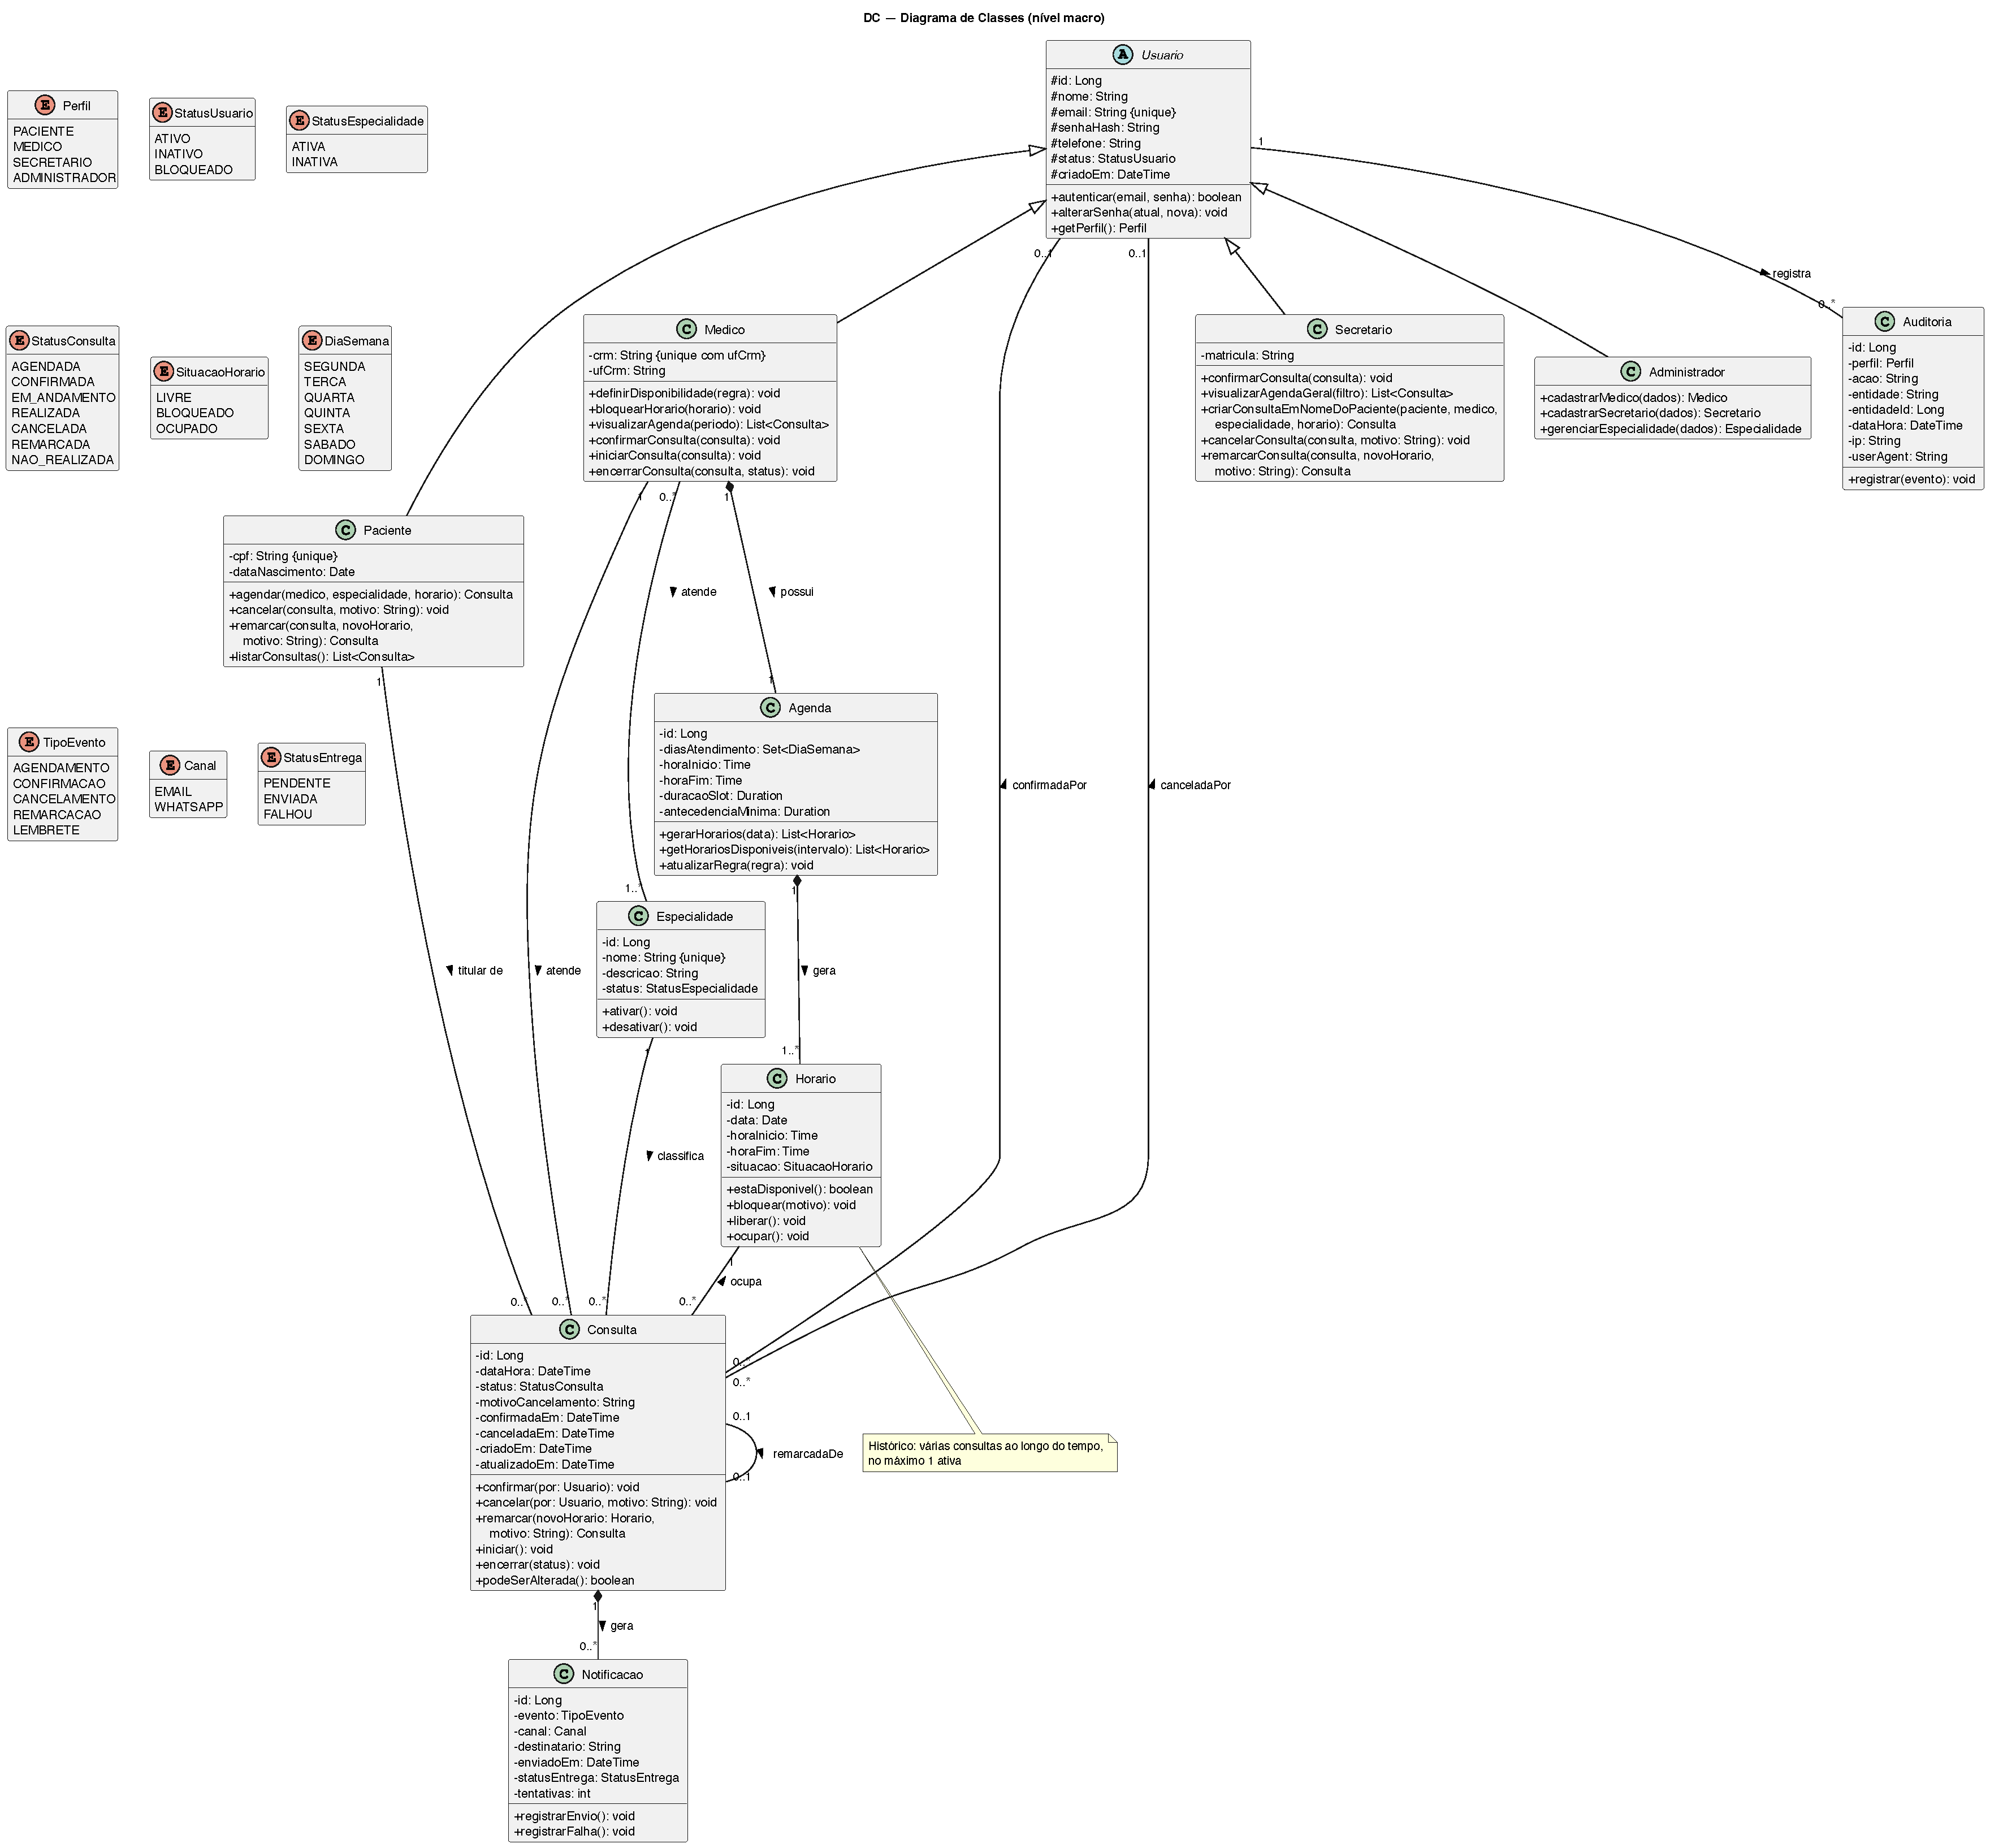
\includegraphics[width=\textwidth,height=0.78\textheight,keepaspectratio]{../assets/DC_Classes.pdf}
\fonte{Elaborado pelos autores (2026).}
\end{figure}

\textbf{Explicação dos elementos:}

Na UML, o símbolo \texttt{+} indica visibilidade pública, \texttt{-}
representa privada e \texttt{\#} indica protegida. Os atributos da
classe \texttt{Usuario} usam \texttt{\#} (protegidos) para permitir que
as subclasses os herdem e acessem diretamente; para as demais classes, o
padrão é manter atributos privados e métodos públicos. Nos
relacionamentos, o losango preenchido marca a composição, o triângulo
vazio indica a herança e a linha simples mostra a associação.

\textbf{Estrutura de Perfis (Herança)}

A classe abstrata \texttt{Usuario} centraliza as informações básicas de
identificação e autenticação (\texttt{id}, \texttt{nome}, \texttt{email},
\texttt{senhaHash}, \texttt{telefone}, \texttt{status} e
\texttt{criadoEm}), além de conter os métodos de segurança. A partir
dela, o sistema se divide em quatro perfis estritos de acesso:

\begin{itemize}
\tightlist
\item
  \textbf{Paciente:} adiciona o atributo \texttt{cpf} ao cadastro.
\item
  \textbf{Medico:} exige as credenciais de \texttt{crm} e \texttt{ufCrm}.
\item
  \textbf{Secretario:} inclui o atributo \texttt{matricula}.
\item
  \textbf{Administrador:} agrupa as operações exclusivas de gestão e
  cadastro da clínica.
\end{itemize}

\textbf{Dependência de Existência (Composição)}

Neste tipo de ligação estrutural, o objeto-todo governa o ciclo de vida
das suas partes:

\begin{itemize}
\tightlist
\item
  \textbf{Medico -- Agenda (1:1):} todo médico possui uma agenda única,
  que perde o sentido e deixa de existir caso o profissional seja
  desvinculado.
\item
  \textbf{Agenda -- Horario (1:1..*):} a agenda fragmenta o expediente em
  slots de atendimento; sem a agenda matriz, esses horários não existem
  de forma autônoma.
\item
  \textbf{Consulta -- Notificacao (1:0..*):} as mensagens pertencem à
  consulta que as originou, mantendo o registro de envios atrelado ao
  evento clínico.
\end{itemize}

\textbf{Vínculos Operacionais (Associações)}

\begin{itemize}
\tightlist
\item
  \textbf{Medico -- Especialidade (0..*:1..*):} um médico atende a uma ou
  múltiplas especialidades, e uma especialidade pode ter vários médicos
  vinculados.
\item
  \textbf{Horario -- Consulta (1:0..*):} um mesmo horário retém o
  histórico de todas as consultas que passaram por ele ao longo do tempo
  (como uma consulta cancelada que cedeu espaço para outra), mas admite no
  máximo uma ativa por vez.
\item
  \textbf{Paciente -- Consulta (1:0..*):} cada consulta pertence
  obrigatoriamente a exatamente um paciente titular, enquanto o paciente
  acumula o histórico de seus agendamentos.
\item
  \textbf{Medico -- Consulta (1:0..*):} cada consulta é conduzida por
  exatamente um médico responsável, enquanto o médico atende a diversas
  consultas na clínica.
\item
  \textbf{Especialidade -- Consulta (1:0..*):} fixa qual especialidade foi
  selecionada no momento da marcação, já que o médico pode atuar em mais
  de uma.
\item
  \textbf{Consulta -- Consulta (0..1:0..1, \texttt{remarcadaDe}):}
  associação reflexiva na qual a nova consulta aponta para a consulta
  anterior cancelada, sendo opcional (\texttt{0..1}) pois agendamentos
  comuns não derivam de outra.
\item
  \textbf{Consulta -- Usuario (0..*:0..1, \texttt{confirmadaPor} e
  \texttt{canceladaPor}):} identifica qual operador executou as ações.
  Cruzando isso com \texttt{confirmadaEm}, \texttt{canceladaEm} e
  \texttt{motivoCancelamento}, obtém-se a rastreabilidade completa do
  ciclo de vida da consulta.
\item
  \textbf{Usuario -- Auditoria (1:0..*):} associação simples (e não
  composição) para assegurar que os logs de auditoria sobrevivam de forma
  imutável e independente da conta do usuário.
\end{itemize}

\textbf{Domínios e Regras (Enumerações)}

\begin{itemize}
\tightlist
\item
  \texttt{Perfil}: trava as contas em \texttt{PACIENTE}, \texttt{MEDICO},
  \texttt{SECRETARIO} ou \texttt{ADMINISTRADOR}.
\item
  \texttt{StatusUsuario}: restringe a situação cadastral a
  \texttt{ATIVO}, \texttt{INATIVO} ou \texttt{BLOQUEADO}.
\item
  \texttt{StatusEspecialidade}: chaveia a disponibilidade no catálogo
  entre \texttt{ATIVA} ou \texttt{INATIVA}.
\item
  \texttt{StatusConsulta}: mapeia o ciclo de atendimento em
  \texttt{AGENDADA}, \texttt{CONFIRMADA}, \texttt{EM\_ANDAMENTO},
  \texttt{REALIZADA}, \texttt{CANCELADA}, \texttt{REMARCADA} ou
  \texttt{NAO\_REALIZADA}.
\item
  \texttt{SituacaoHorario}: controla o estado de cada vaga da grade como
  \texttt{LIVRE}, \texttt{BLOQUEADO} ou \texttt{OCUPADO}.
\item
  \texttt{DiaSemana}: parametriza os dias de atendimento configurados na
  agenda do médico.
\item
  \texttt{TipoEvento}: filtra os gatilhos de comunicação em
  \texttt{AGENDAMENTO}, \texttt{CONFIRMACAO}, \texttt{CANCELAMENTO},
  \texttt{REMARCACAO} ou \texttt{LEMBRETE}.
\item
  \texttt{Canal}: limita os disparos de notificação a \texttt{EMAIL} ou
  \texttt{WHATSAPP}.
\item
  \texttt{StatusEntrega}: sinaliza o resultado do envio via
  \texttt{PENDENTE}, \texttt{ENVIADA} ou \texttt{FALHOU}.
\end{itemize}

\section{Considerações Finais}\label{sec:consideracoes}

A modelagem desenvolvida mostra como a UML organiza e comunica a
estrutura e o comportamento de um sistema antes da implementação,
conectando as regras de negócio aos modelos de software.

O \textbf{diagrama de atividades} (DA-01) descreve o processo de
agendamento de ponta a ponta. Com raias para o paciente, o sistema e o
Sistema de Notificação, ele cobre o fluxo principal e todos os fluxos
alternativos e de exceção (sem vagas, horário ocupado, horário fora da
janela, sessão expirada, falha de gravação e falha de notificação) e usa
\emph{fork/join} (divisão e junção de fluxos paralelos) em dois níveis:
no primeiro, o comprovante é gerado em paralelo ao envio das
notificações; no segundo, dentro do envio, o e-mail e o WhatsApp saem em
paralelo, cada um com suas próprias tentativas.

O \textbf{diagrama de sequência} (DS-01) mostra, no mesmo cenário, a
troca de mensagens ao longo do tempo. Seus destaques são a reserva
atômica do horário, ou seja, de uma só vez, sem risco de dois pacientes
ficarem com o mesmo horário; o \emph{rollback} (desfazer a operação) em
caso de falha; a criação da consulta e o envio assíncrono e paralelo por
e-mail e WhatsApp, com até 3 tentativas em cada canal.

O \textbf{diagrama de classes} estrutura a visão estática do domínio com
11 classes e 9 enumerações, relacionamentos de herança, composição e
associação com multiplicidades, e indica a visibilidade dos atributos e
métodos.

Todos os diagramas foram revisados para garantir que estivessem
coerentes entre si. Dessa revisão resultaram decisões que tornaram o
modelo mais fiel às regras de negócio, como a multiplicidade entre
\texttt{Horario} e \texttt{Consulta}, o registro de quem confirmou e
quem cancelou, a reserva atômica do horário e a separação entre o
comprovante e o envio da notificação.

\textbf{Limitações e próximos passos:} a remarcação, a confirmação pelo
secretário e o cancelamento estão descritos em texto
(seções~\ref{sec:modulos-regras} e~\ref{sec:ciclo}), mas não têm
diagrama próprio, porque o DA-01 e o DS-01 já cobrem o que foi pedido.
Se houver evolução do trabalho, esses cenários são os candidatos
naturais a novos diagramas (por exemplo, o cancelamento com bloqueio da
janela de 2 horas).

% =========================================================================
% ELEMENTOS PÓS-TEXTUAIS (NBR 14724 / NBR 6023)
% =========================================================================

\newpage
\phantomsection
\addcontentsline{toc}{section}{REFERÊNCIAS}
\section*{REFERÊNCIAS}

\begin{singlespace}
\setlength{\parindent}{0pt}
\setlength{\parskip}{1.5ex}

FOWLER, Martin. \textbf{UML essencial}: um breve guia para a linguagem-padrão de modelagem de objetos. 3.~ed. Porto Alegre: Bookman, 2005.

OBJECT MANAGEMENT GROUP (OMG). \textbf{OMG Unified Modeling Language (OMG UML)}: Superstructure, Version 2.5.1. Needham: OMG, 2017. Disponível em: \url{https://www.omg.org/spec/UML/2.5.1/}. Acesso em: 8 out. 2026.

PLANTUML. \textbf{PlantUML Language Reference Guide}. 2024. Disponível em: \url{https://plantuml.com/guide}. Acesso em: 8 out. 2026.

PRESSMAN, Roger S.; MAXIM, Bruce R. \textbf{Engenharia de software}: uma abordagem profissional. 8.~ed. Porto Alegre: AMGH, 2016.

SOMMERVILLE, Ian. \textbf{Engenharia de software}. 10.~ed. São Paulo: Pearson Education do Brasil, 2019.

\end{singlespace}

\newpage
\appendix

% Rótulo "APÊNDICE A --" apenas para as seções pós-textuais
\titleformat{\section}
  {\normalfont\normalsize\bfseries\MakeUppercase}{APÊNDICE~\thesection~---}{1em}{}

\section{Especificação de Requisitos e Regras de Negócio}\label{sec:apendice}

As decisões de modelagem apresentadas neste trabalho foram fundamentadas
em um levantamento prévio de requisitos funcionais e regras de negócio,
consolidados abaixo para fins de consulta e rastreabilidade.

\subsection{Requisitos Funcionais (RF)}\label{sec:rf}

\subsubsection{Módulo de Cadastro e Autenticação}

\begin{table}[H]
\centering
{\footnotesize
\begin{tabularx}{\textwidth}{@{}c>{\raggedright\arraybackslash}p{2.9cm}>{\raggedright\arraybackslash}X>{\raggedright\arraybackslash}p{2.7cm}@{}}
\toprule
ID & Requisito & Descrição & Regras relacionadas \\
\midrule
RF-01 & Cadastrar paciente & O sistema deve permitir o cadastro de paciente com nome, CPF, data de nascimento, e-mail, telefone e senha. & RN-01, RN-02, RN-03 \\
RF-02 & Autenticar usuário & O sistema deve autenticar paciente, médico, secretário e administrador por e-mail + senha, diferenciando perfis. & RN-04, RN-06 \\
RF-03 & Recuperar senha & O sistema deve permitir redefinição de senha por link enviado ao e-mail cadastrado. & RN-05 \\
RF-04 & Gerenciar cadastro de médico e secretário & O \textbf{Administrador} deve poder cadastrar médico (nome, CRM, UF, especialidade(s) e contato) e secretário (nome, matrícula e contato). & RN-02, RN-07, RN-08 \\
RF-05 & Gerenciar especialidades & O \textbf{Administrador} deve poder manter o catálogo de especialidades (nome, descrição, status ATIVA/INATIVA). & RN-09 \\
\bottomrule
\end{tabularx}
}
\fonte{Elaborado pelos autores (2026).}
\end{table}

\subsubsection{Módulo de Consulta de Médicos e Especialidades}

\begin{table}[H]
\centering
{\footnotesize
\begin{tabularx}{\textwidth}{@{}c>{\raggedright\arraybackslash}p{2.9cm}>{\raggedright\arraybackslash}X>{\raggedright\arraybackslash}p{2.7cm}@{}}
\toprule
ID & Requisito & Descrição & Regras relacionadas \\
\midrule
RF-06 & Listar especialidades & O sistema deve exibir todas as especialidades ativas para busca. & RN-09 \\
RF-07 & Listar médicos por especialidade & Dada uma especialidade, o sistema deve listar os médicos ativos que a atendem. & RN-07, RN-10 \\
RF-08 & Exibir horários disponíveis & Para cada médico, o sistema deve exibir apenas os horários \textbf{livres} dentro da sua disponibilidade, considerando o horário atual. & RN-11, RN-12, RN-13 \\
\bottomrule
\end{tabularx}
}
\fonte{Elaborado pelos autores (2026).}
\end{table}

\subsubsection{Módulo de Agendamento}

\begin{table}[H]
\centering
{\footnotesize
\begin{tabularx}{\textwidth}{@{}c>{\raggedright\arraybackslash}p{2.9cm}>{\raggedright\arraybackslash}X>{\raggedright\arraybackslash}p{2.7cm}@{}}
\toprule
ID & Requisito & Descrição & Regras relacionadas \\
\midrule
RF-09 & Agendar consulta & O paciente deve poder agendar consulta selecionando especialidade $\rightarrow$ médico $\rightarrow$ data $\rightarrow$ horário livre, com confirmação final antes do envio. & RN-10, RN-11, RN-13, RN-16, RN-18 \\
RF-10 & Confirmar agendamento & Após a reserva bem-sucedida, o sistema deve exibir resumo da consulta e disparar notificação de agendamento. & RN-25, RN-27 \\
RF-11 & Visualizar minhas consultas & O paciente deve poder listar suas consultas futuras e passadas com respectivo status. & RN-19 \\
RF-12 & Cancelar consulta & O paciente (ou secretário) deve poder cancelar uma consulta futura, informando o motivo (obrigatório), liberando o horário. & RN-20, RN-21 \\
RF-13 & Remarcar consulta & O paciente titular (ou o secretário) deve poder remarcar uma consulta futura \textbf{com o mesmo médico}, informando o motivo (obrigatório) e validando o novo horário como uma nova reserva. & RN-13, RN-17, RN-20, RN-21 \\
RF-22 & Agir em nome do paciente & O secretário deve poder agendar, remarcar e cancelar consultas em nome de um paciente cadastrado (atendimento presencial/telefônico), com as mesmas validações de RF-09, RF-12 e RF-13. & RN-10, RN-11, RN-13, RN-16, RN-18, RN-20, RN-23 \\
\bottomrule
\end{tabularx}
}
\fonte{Elaborado pelos autores (2026).}
\end{table}

\subsubsection{Módulo de Agenda do Médico}

\begin{table}[H]
\centering
{\footnotesize
\begin{tabularx}{\textwidth}{@{}c>{\raggedright\arraybackslash}p{2.9cm}>{\raggedright\arraybackslash}X>{\raggedright\arraybackslash}p{2.7cm}@{}}
\toprule
ID & Requisito & Descrição & Regras relacionadas \\
\midrule
RF-14 & Definir disponibilidade & O médico deve poder definir dias da semana e faixas horárias de atendimento, com antecedência mínima configurável. & RN-11, RN-12, RN-13, RN-15 \\
RF-15 & Bloquear horário & O médico deve poder bloquear um horário específico já disponível (sem consulta), tornando-o indisponível. O secretário pode registrar bloqueios operacionais justificados. & RN-14, RN-15 \\
RF-16 & Visualizar agenda & O médico e o secretário devem poder visualizar a agenda em visão diária/semanal, com status de cada consulta. & RN-19 \\
RF-17 & Atender e encerrar consulta & O médico deve poder iniciar a consulta, marcá-la como \textbf{realizada} ao final do atendimento ou registrar a \textbf{ausência} do paciente (\texttt{NAO\_REALIZADA}). & RN-22, RN-24 \\
\bottomrule
\end{tabularx}
}
\fonte{Elaborado pelos autores (2026).}
\end{table}

\subsubsection{Módulo de Confirmação (Secretário)}

\begin{table}[H]
\centering
{\footnotesize
\begin{tabularx}{\textwidth}{@{}c>{\raggedright\arraybackslash}p{2.9cm}>{\raggedright\arraybackslash}X>{\raggedright\arraybackslash}p{2.7cm}@{}}
\toprule
ID & Requisito & Descrição & Regras relacionadas \\
\midrule
RF-18 & Confirmar consulta & O secretário (ou o médico titular) deve poder confirmar uma consulta com status \textit{agendada}, alterando-a para \textit{confirmada} e registrando quem confirmou e quando. & RN-24, RN-25, RN-26 \\
RF-19 & Visualizar pendências & O sistema deve listar as consultas pendentes de confirmação, filtráveis por médico, data e status. & RN-26 \\
\bottomrule
\end{tabularx}
}
\fonte{Elaborado pelos autores (2026).}
\end{table}

\subsubsection{Módulo de Notificação}

\begin{table}[H]
\centering
{\footnotesize
\begin{tabularx}{\textwidth}{@{}c>{\raggedright\arraybackslash}p{2.9cm}>{\raggedright\arraybackslash}X>{\raggedright\arraybackslash}p{2.7cm}@{}}
\toprule
ID & Requisito & Descrição & Regras relacionadas \\
\midrule
RF-20 & Notificar eventos & O sistema deve disparar notificações nos eventos: agendada, confirmada, cancelada, remarcada, lembrete pré-consulta. & RN-25, RN-27, RN-28 \\
RF-21 & Registrar notificações & Cada notificação deve ser persistida com destinatário, evento, canal, data/hora e status de entrega. & RN-27 \\
\bottomrule
\end{tabularx}
}
\fonte{Elaborado pelos autores (2026).}
\end{table}

\subsection{Regras de Negócio (RN)}\label{sec:rn}

\subsubsection{Identificação e acesso}

\begin{table}[H]
\centering
{\footnotesize
\begin{tabularx}{\textwidth}{@{}>{\raggedright\arraybackslash}p{1.8cm}>{\raggedright\arraybackslash}X@{}}
\toprule
ID & Regra \\
\midrule
\textbf{RN-01} & O CPF deve ter 11 dígitos, ser válido (módulo 11) e \textbf{único} no cadastro de pacientes. \\
\textbf{RN-02} & O e-mail deve ser válido e \textbf{único} por usuário no sistema. \\
\textbf{RN-03} & A senha deve ter no mínimo 8 caracteres, contendo ao menos 1 letra e 1 número. \\
\textbf{RN-04} & O sistema autentica por e-mail + senha e deriva o perfil (PACIENTE, MEDICO, SECRETARIO, ADMINISTRADOR) do cadastro. \\
\textbf{RN-05} & Links de redefinição de senha expiram em 30 minutos e são de uso único. \\
\textbf{RN-06} & Após 5 falhas consecutivas de login, a conta é bloqueada por 15 minutos. \\
\bottomrule
\end{tabularx}
}
\fonte{Elaborado pelos autores (2026).}
\end{table}

\subsubsection{Cadastros e catálogo}

\begin{table}[H]
\centering
{\footnotesize
\begin{tabularx}{\textwidth}{@{}>{\raggedright\arraybackslash}p{1.8cm}>{\raggedright\arraybackslash}X@{}}
\toprule
ID & Regra \\
\midrule
\textbf{RN-07} & Todo médico deve ter \textbf{ao menos uma} especialidade ativa para aparecer nas buscas. \\
\textbf{RN-08} & O par (CRM, UF) do médico é \textbf{único} no sistema. \\
\textbf{RN-09} & Só são exibidas especialidades com \texttt{status = ATIVA}. \\
\textbf{RN-10} & Paciente, médico, secretário e administrador só são exibidos com \texttt{status = ATIVO}; cadastro inativo não pode gerar novas consultas. \\
\bottomrule
\end{tabularx}
}
\fonte{Elaborado pelos autores (2026).}
\end{table}

\subsubsection{Disponibilidade e horários}

\begin{table}[H]
\centering
{\footnotesize
\begin{tabularx}{\textwidth}{@{}>{\raggedright\arraybackslash}p{1.8cm}>{\raggedright\arraybackslash}X@{}}
\toprule
ID & Regra \\
\midrule
\textbf{RN-11} & Um horário só é considerado \textbf{disponível} se: pertencer à disponibilidade do médico, estar dentro do expediente configurado, não estiver bloqueado e \textbf{não houver consulta ativa} (AGENDADA, CONFIRMADA ou EM\_ANDAMENTO) naquele slot. \\
\textbf{RN-12} & Cada consulta ocupa \textbf{um slot} de \textbf{30 minutos por padrão} (configurável pelo médico em múltiplos de 30), sem sobreposição entre consultas do mesmo médico. \\
\textbf{RN-13} & Só é permitido agendar a partir de \texttt{agora + antecedênciaMinima} da agenda do médico (\textbf{padrão 30 min}) e com no máximo \textbf{90 dias} de antecedência. \\
\textbf{RN-14} & Bloqueios operacionais de horário feitos pelo secretário exigem justificativa e ficam registrados em auditoria. \\
\textbf{RN-15} & Alterações de disponibilidade ou bloqueios que atinjam consultas já existentes \textbf{não} as cancelam automaticamente; o sistema deve sinalizar conflito e exigir tratamento manual. \\
\bottomrule
\end{tabularx}
}
\fonte{Elaborado pelos autores (2026).}
\end{table}

\subsubsection{Ciclo de vida da consulta}

\begin{table}[H]
\centering
{\footnotesize
\begin{tabularx}{\textwidth}{@{}>{\raggedright\arraybackslash}p{1.8cm}>{\raggedright\arraybackslash}X@{}}
\toprule
ID & Regra \\
\midrule
\textbf{RN-16} & Toda consulta nasce com status \texttt{AGENDADA} e está sempre associada a \textbf{1 paciente, 1 médico, 1 especialidade e 1 slot de horário}. \\
\textbf{RN-17} & A \textbf{remarcação} é modelada como: cancelamento da consulta original (status \texttt{REMARCADA}, com vínculo para a nova) + criação de nova consulta. A remarcação mantém o \textbf{mesmo médico}; trocar de médico exige cancelar e agendar novamente. \\
\textbf{RN-18} & Apenas uma consulta pode ocupar o mesmo (médico, data, horário) com status ativo; consultas canceladas ou remarcadas permanecem como histórico, vinculadas ao mesmo \texttt{Horario}. \\
\textbf{RN-19} & Consultas \texttt{AGENDADA} ou \texttt{CONFIRMADA} cujo slot terminou sem terem sido iniciadas transicionam automaticamente para \texttt{NAO\_REALIZADA} (executado pelo Sistema/agendador). \\
\textbf{RN-20} & Cancelamento/remarcação só é permitido \textbf{até 2 horas antes} do horário da consulta. \\
\textbf{RN-21} & Cancelamentos e remarcações exigem \textbf{confirmação explícita} do usuário, registram autor (\texttt{canceladaPor}) e data (\texttt{canceladaEm}), e exigem \textbf{motivo obrigatório} (\texttt{motivoCancelamento}). \\
\textbf{RN-22} & Somente o médico titular pode iniciar, encerrar (\texttt{REALIZADA}) ou registrar ausência (\texttt{NAO\_REALIZADA}) de uma consulta. \texttt{REALIZADA} só é alcançado a partir de \texttt{EM\_ANDAMENTO}. \\
\textbf{RN-23} & Consulta criada, remarcada ou cancelada pelo secretário em nome do paciente registra o secretário como autor na auditoria e notifica o paciente conforme RN-25. \\
\textbf{RN-24} & A confirmação (\texttt{CONFIRMADA}) é \textbf{opcional}: o médico pode iniciar uma consulta \texttt{AGENDADA} ou \texttt{CONFIRMADA}. \\
\bottomrule
\end{tabularx}
}
\fonte{Elaborado pelos autores (2026).}
\end{table}

\subsubsection{Confirmação e notificação}

\begin{table}[H]
\centering
{\footnotesize
\begin{tabularx}{\textwidth}{@{}>{\raggedright\arraybackslash}p{1.8cm}>{\raggedright\arraybackslash}X@{}}
\toprule
ID & Regra \\
\midrule
\textbf{RN-25} & Cada evento de negócio (\texttt{AGENDAMENTO}, \texttt{CONFIRMACAO}, \texttt{CANCELAMENTO}, \texttt{REMARCACAO}) dispara uma notificação por destinatário \textbf{e por canal} (e-mail e WhatsApp). Mudanças para \texttt{EM\_ANDAMENTO}, \texttt{REALIZADA} e \texttt{NAO\_REALIZADA} não geram notificação. \\
\textbf{RN-26} & Somente \textbf{secretário} ou o \textbf{médico titular} pode confirmar consulta; a confirmação registra o autor (\texttt{confirmadaPor}) e o timestamp (\texttt{confirmadaEm}). \\
\textbf{RN-27} & Falha no envio de notificação \textbf{não} desfaz a transação principal; a notificação entra em fila de nova tentativa (até 3 tentativas com backoff). Cada canal tem o seu registro de \texttt{Notificacao} e as suas tentativas. \\
\textbf{RN-28} & O lembrete é disparado \textbf{24 h antes} do horário da consulta, apenas para status \texttt{CONFIRMADA} ou \texttt{AGENDADA}. \\
\bottomrule
\end{tabularx}
}
\fonte{Elaborado pelos autores (2026).}
\end{table}

\newpage
\section{Código-fonte PlantUML dos Diagramas}\label{sec:apendice-codigo}

Os diagramas apresentados neste trabalho foram elaborados em PlantUML. Os
códigos-fonte que geraram os modelos são reproduzidos a seguir para fins
de verificação e reprodutibilidade.

\subsection{DA-01 --- Agendamento de Consulta}

\lstinputlisting{../assets/DA01_Agendamento.puml}
\fonte{Elaborado pelos autores (2026).}

\subsection{DS-01 --- Agendamento de Consulta (Fluxo Completo)}

\lstinputlisting{../assets/DS01_Agendamento.puml}
\fonte{Elaborado pelos autores (2026).}

\subsection{DC --- Diagrama de Classes (Nível Macro)}

\lstinputlisting{../assets/DC_Classes.puml}
\fonte{Elaborado pelos autores (2026).}

\end{document}
